\chapter{De to Algoritmer}
\label{ch:De to Algoritmer}

\section{Insertionsort}
\label{sec:Insertionsort}

Insertionsort implementeret i python:

\lstinputlisting[language=Python]{../python/algoritmer/insertionsort.py}

\subsection{Analyse af Insertionsort}
\label{sec:Analyse af Insertionsort}
Funktionen for køretiden af denne algoritme er en del af mængden $O(n^2)$.


\section{Mergesort}
\label{sec:Mergesort}

Mergesort implementeret i python \cite[s. 106]{aogd}:
\lstinputlisting[language=Python]{../python/algoritmer/mergesort.py}

\section{Sammenligning af Algoritmerne}
\label{sec:Sammenligninng af Algoritmerne}


\begin{figure}
	\centering
	\begin{subfigure}[b]{0.45\textwidth}
		\centering
		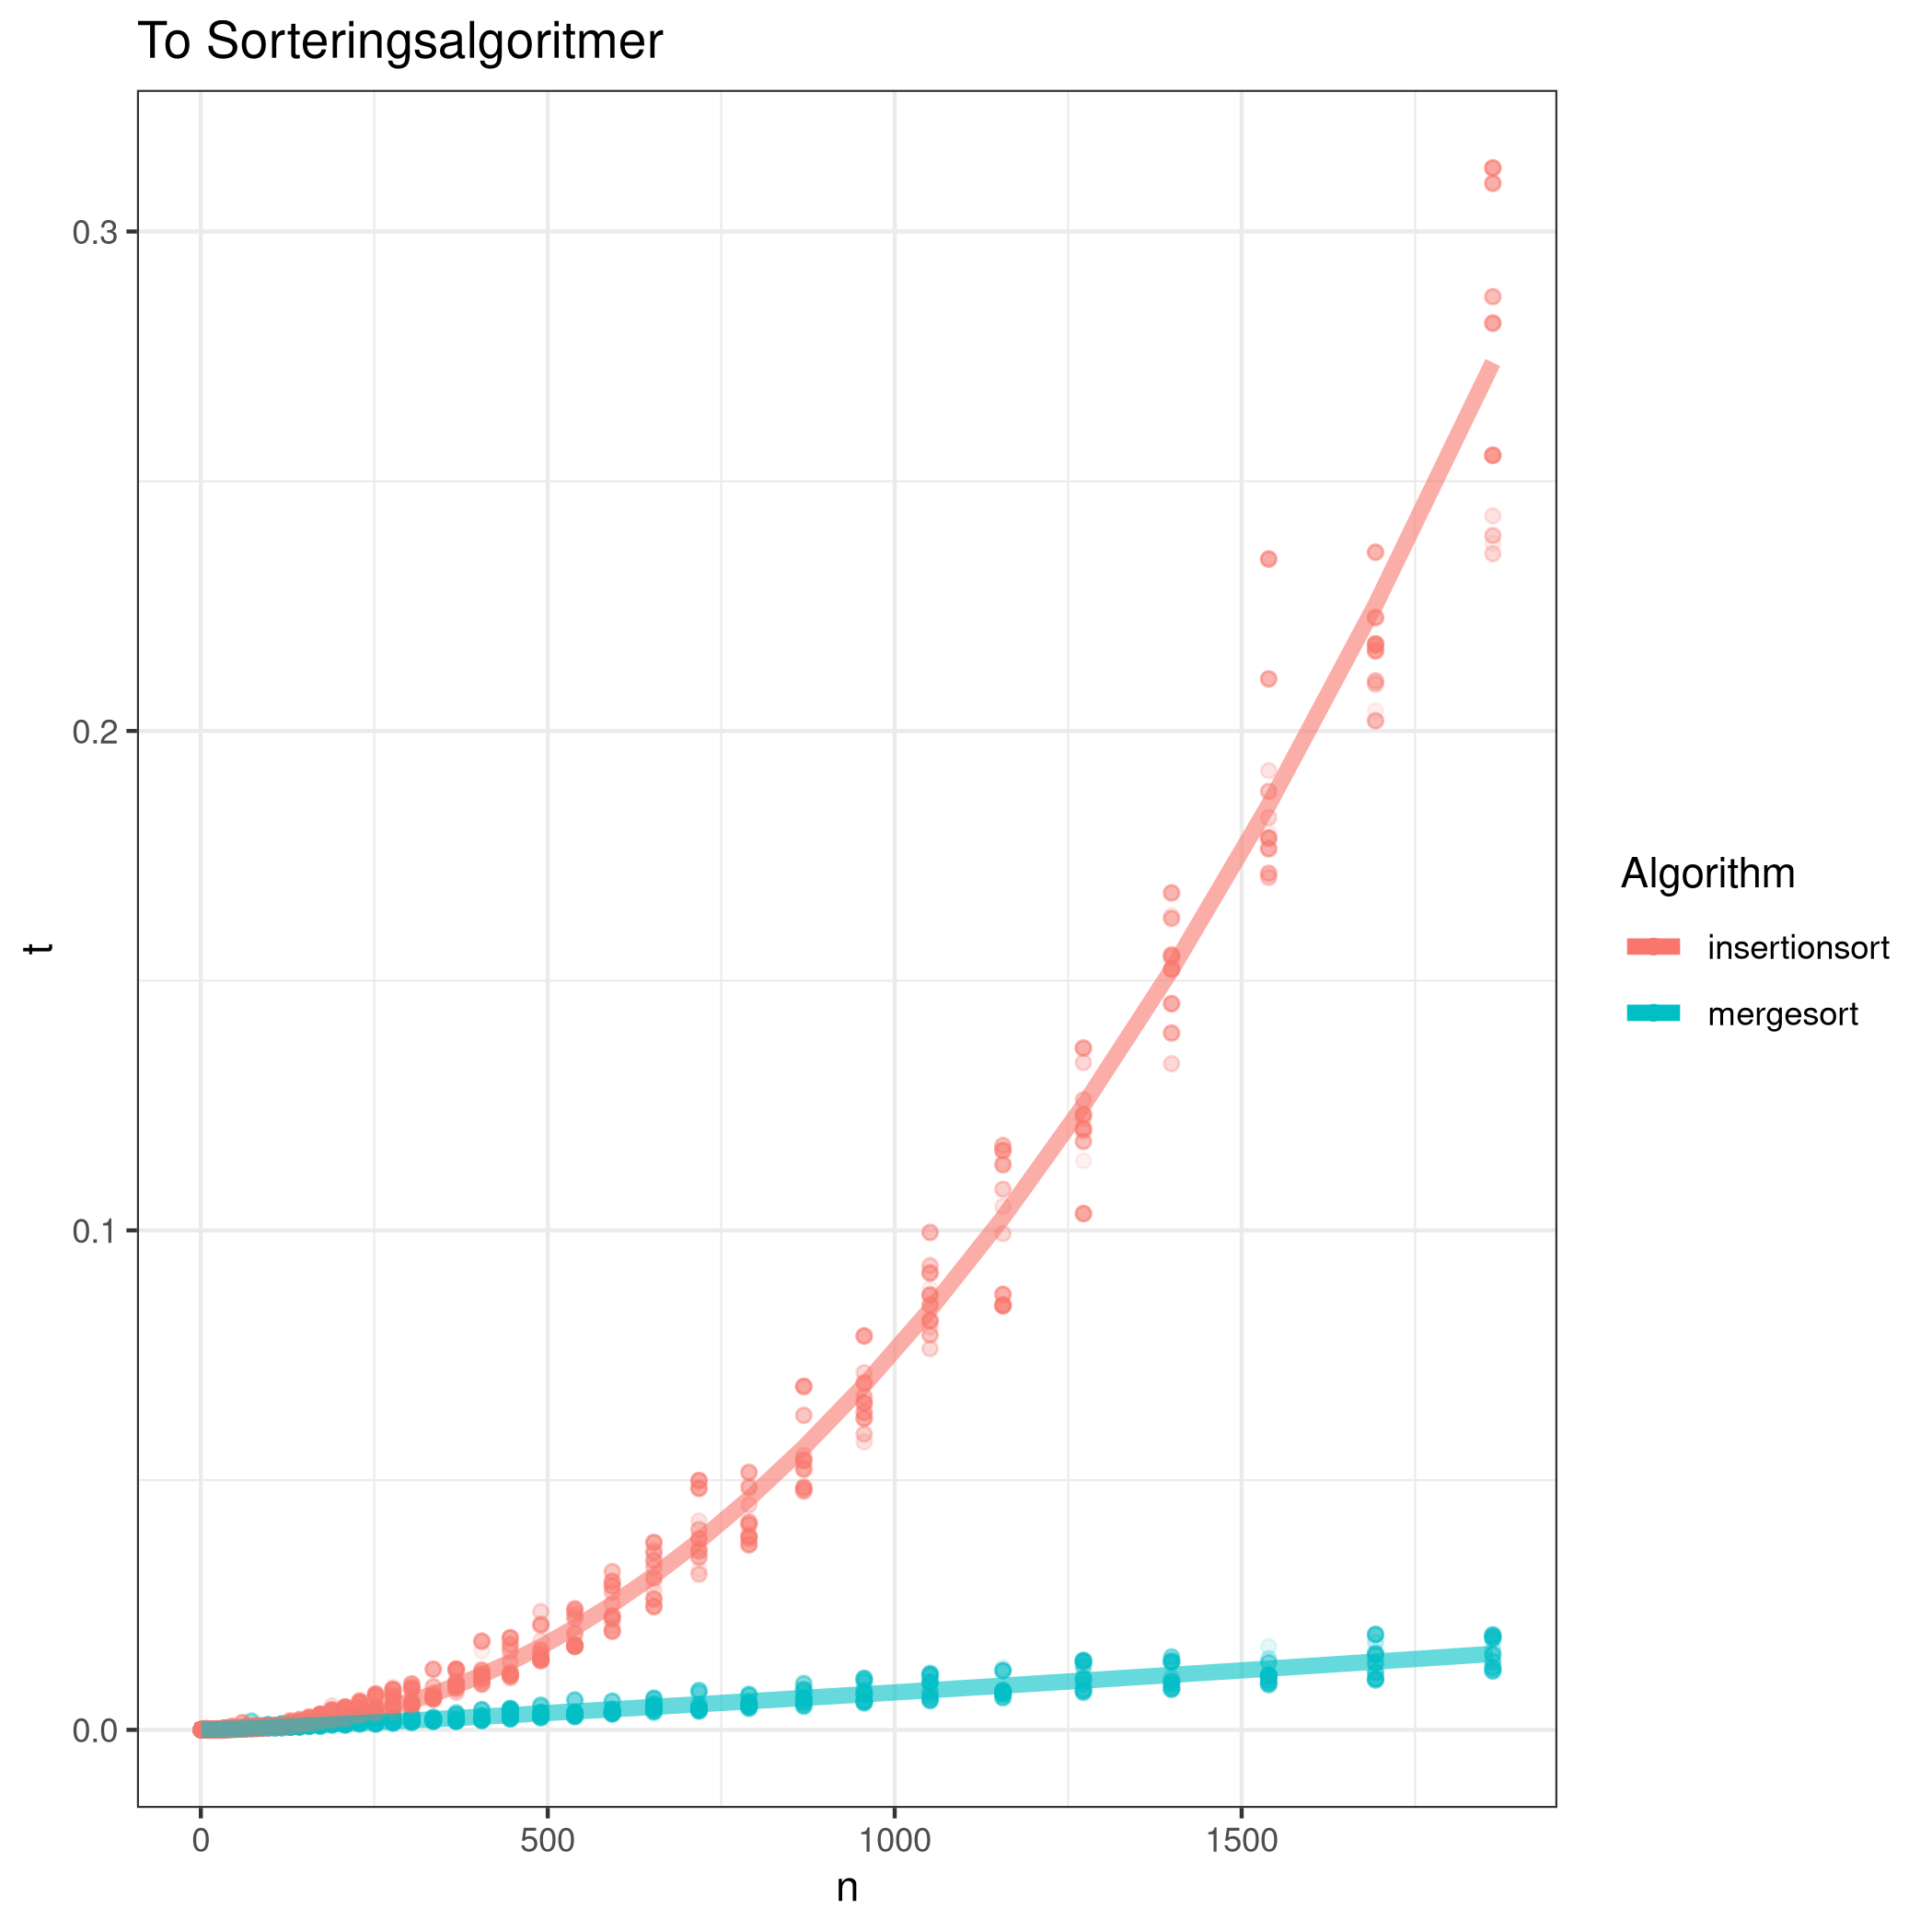
\includegraphics[width=\textwidth]{../img/toAlgoritmer.png}
		\caption{$y=\input{../img/r2-insertion.txt}$}
		\label{fig:regressioner}
	\end{subfigure}
	\hfill
	\begin{subfigure}[b]{0.45\textwidth}
		\centering
		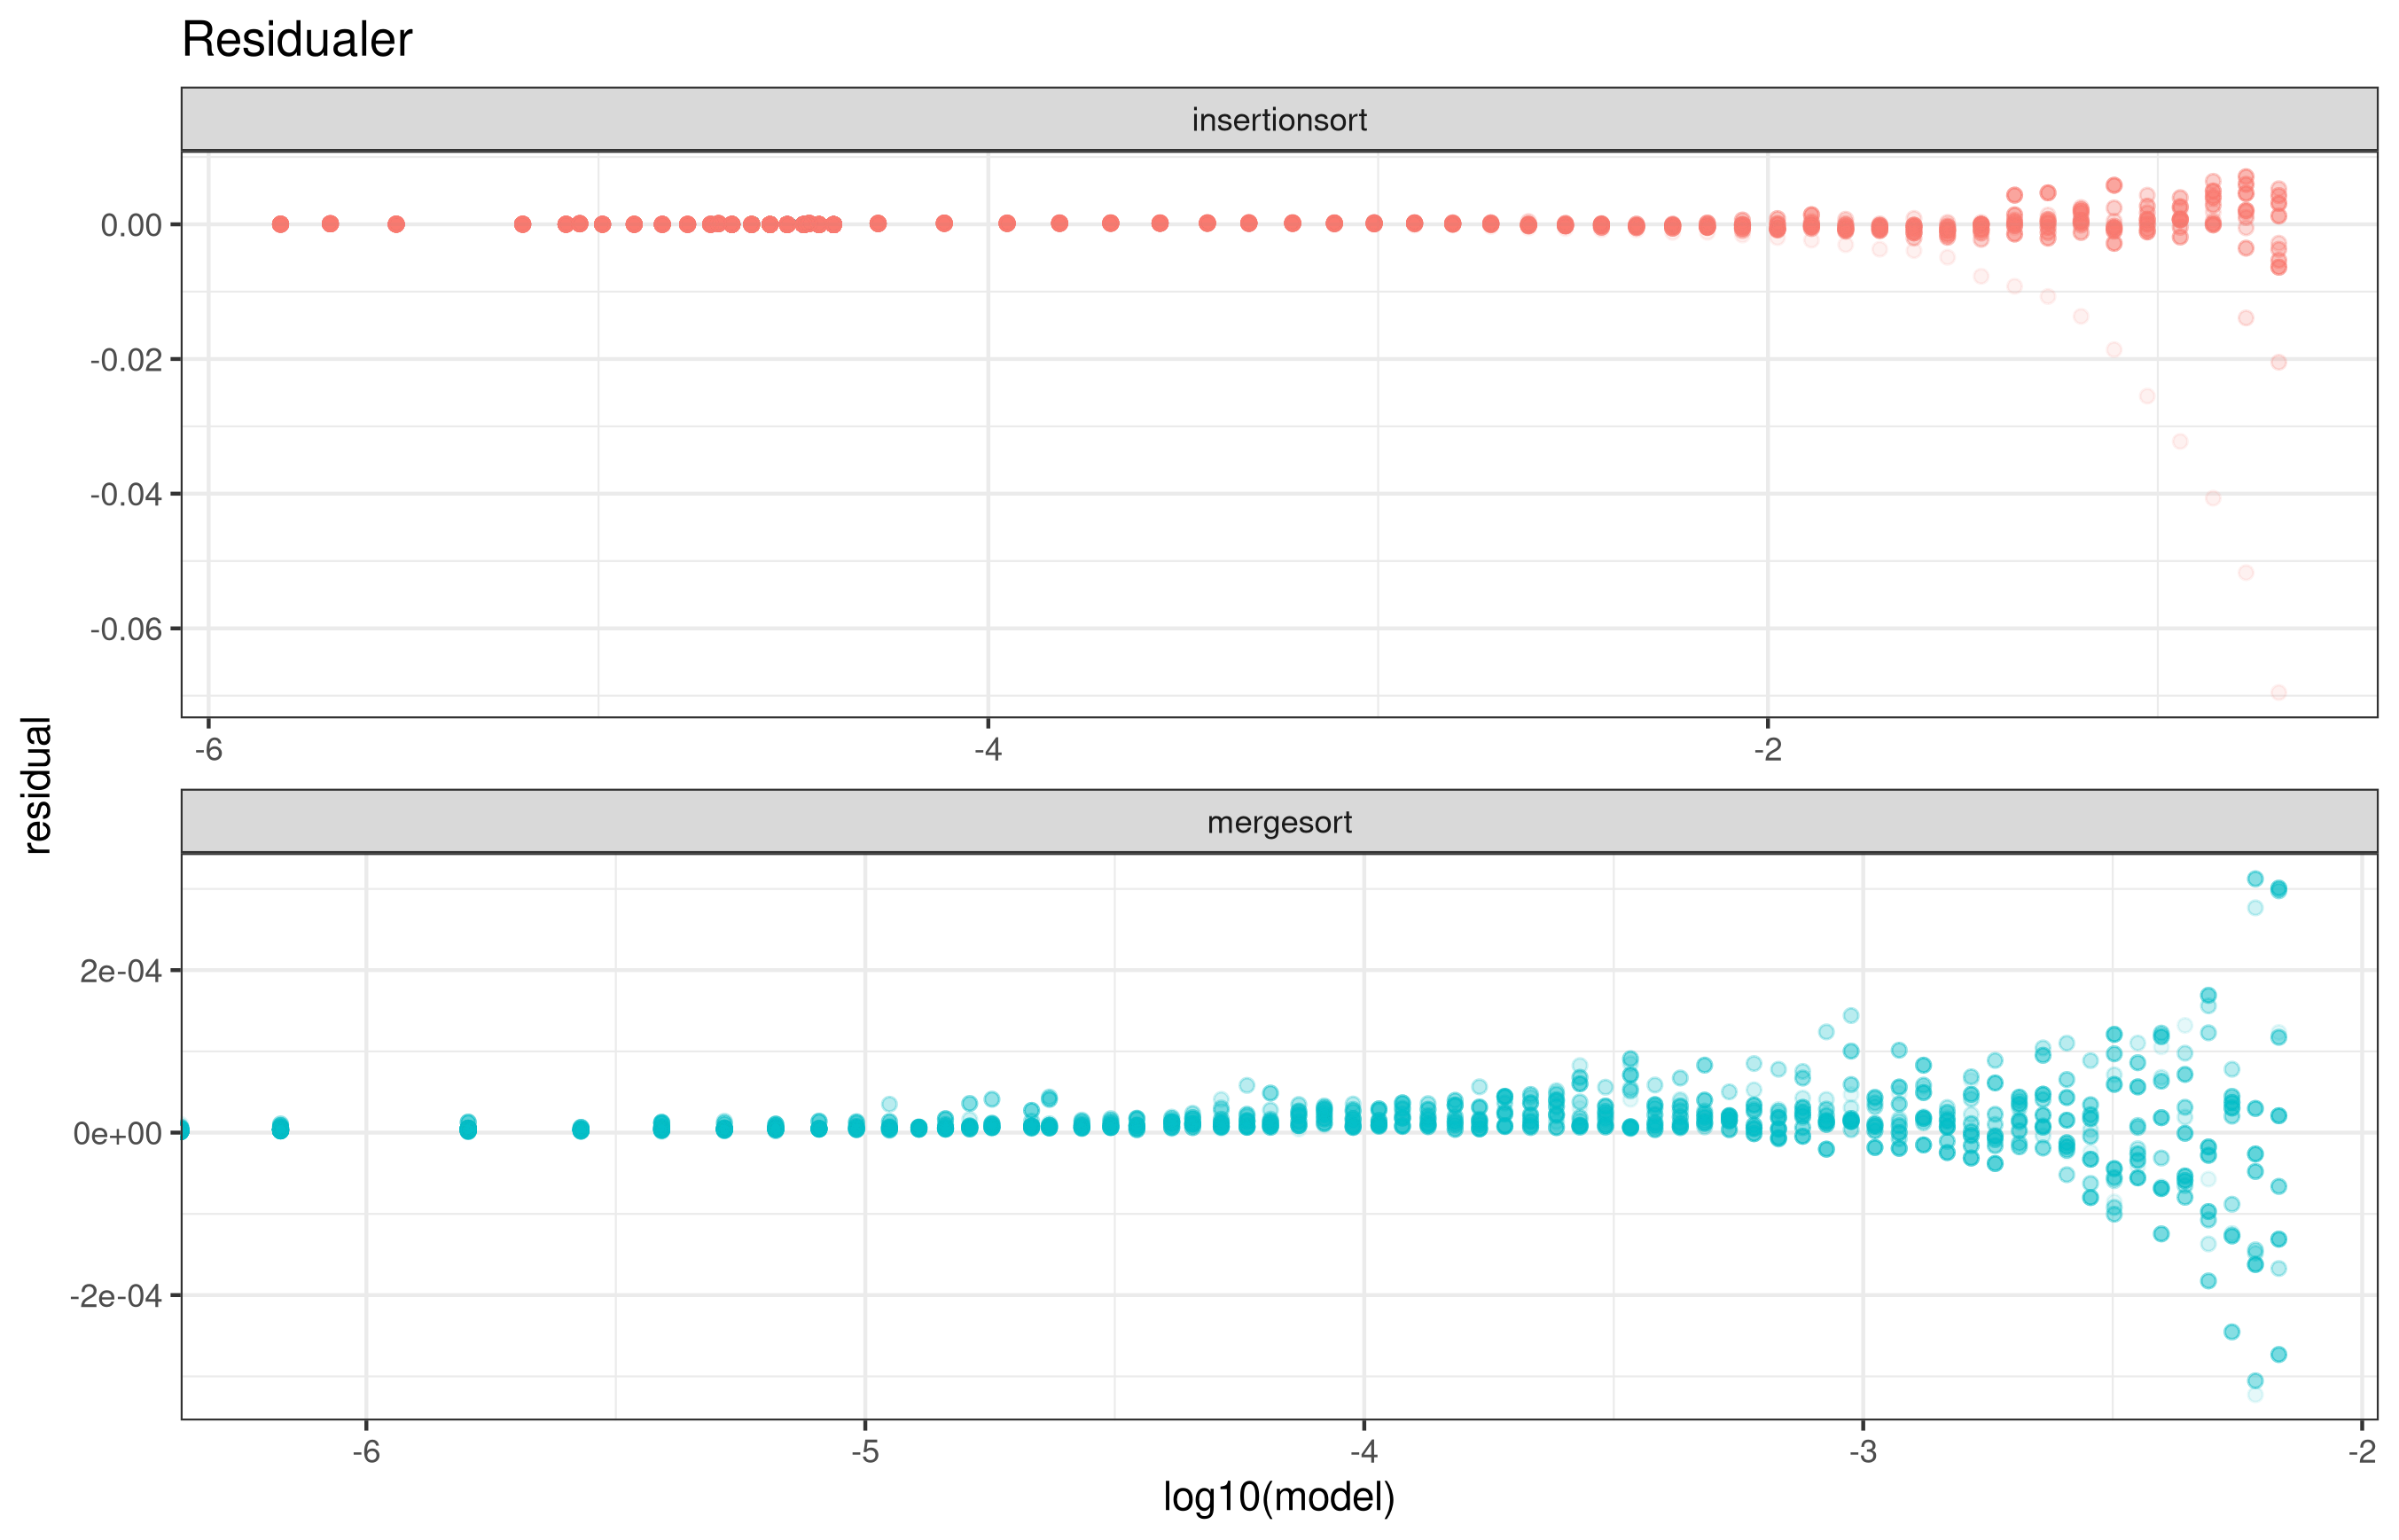
\includegraphics[width=\textwidth]{../img/toAlgoritmerResidual}
		\caption{$y=3sinx$}
		\label{fig:residualplot}
	\end{subfigure}
	\caption{Sammenligning af insertionsort og mergesort}
	\label{toAlgoritmer}
\end{figure}

\section{Den Optimerede Mergesort}
\label{sec:Den Optimerede Mergesort}





